\documentclass[cn,10pt,math=newtx,citestyle=gb7714-2015,bibstyle=gb7714-2015]{elegantbook}

%latex 宏
% 书签
\usepackage{bookmark}
% 画图
\usepackage{tikz}
% 图片
\usepackage{graphicx}
\usepackage{caption}
\usepackage{subfigure}
\usepackage{float}
% 代码块
\usepackage{listings}
\definecolor{GreenBlue}{RGB}{31,144,144}
\definecolor{NavyBlue}{RGB}{78,112,224}
\definecolor{BurntOrange}{RGB}{192,144,31}
\definecolor{ForestGreen}{RGB}{78,144,78}
\definecolor{Purple}{RGB}{112,78,144}

\lstdefinelanguage{Kotlin}{
  comment=[l]{//},
  commentstyle={\color{gray}\ttfamily},
  emph={filter, first, firstOrNull, forEach, lazy, map, mapNotNull, println},
  emphstyle={\color{GreenBlue}\textit},
  identifierstyle=\color{black},
  keywords={!in, !is, abstract, actual, annotation, as, as?, break, by, catch, class, companion, const, constructor, continue, crossinline, data, delegate, do, dynamic, else, enum, expect, external, false, field, file, final, finally, for, fun, get, if, import, in, infix, init, inline, inner, interface, internal, is, lateinit, noinline, null, object, open, operator, out, override, package, param, private, property, protected, public, receiveris, reified, return, return@, sealed, set, setparam, super, suspend, tailrec, this, throw, true, try, typealias, typeof, val, var, vararg, when, where, while, implements, extends},
  keywordstyle={\color{NavyBlue}\bfseries},
  morecomment=[s]{/*}{*/},
  morestring=[b]",
  morestring=[s]{"""*}{*"""},
  ndkeywords={@Deprecated, @JvmField, @JvmName, @JvmOverloads, @JvmStatic, @JvmSynthetic, @Test, @Override, Array, Byte, Double, Float, Int, Integer, Iterable, Long, Runnable, Short, String},
  ndkeywordstyle={\color{BurntOrange}\bfseries},
  sensitive=true,
  stringstyle={\color{ForestGreen}\ttfamily},
  numbers = left,   % 行号的位置在左边
  numberstyle={\color{Purple}\ttfamily}
}

\def\degree{${}^{\circ}$}

%region 元数据声明
\title{编程笔记}

\author{igrape}
\institute{TropicalTeamYard}
\date{2021年7月10日}
\version{0.1}

\extrainfo{各人自扫门前雪,休管他人瓦上霜。—— 陈元靓}

\setcounter{tocdepth}{3}

\cover{images/cover.jpg}




%endregion
\begin{document}
    \maketitle

    \frontmatter

    \chapter*{特别声明}

    \markboth{Introduction}{前言}

    编程笔记

    \begin{flushright}
    igrape \\
    2021年7月10日
    \end{flushright}
    
    \tableofcontents

    \mainmatter

    \chapter{Java\&Kotlin}

    \section{Joda-time时间处理类(since 1.8)\label{section_1}}

    \begin{flushright}
        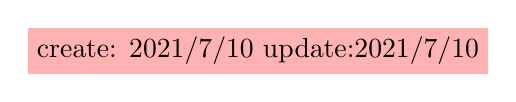
\begin{tikzpicture}
            \draw (0,0) node [fill=red!30!white] {create: 2021/7/10 update:2021/7/10};
        \end{tikzpicture}
    \end{flushright}

    \subsection{简介}

    在Kotlin中处理日期和时间是很常见的需求,在Java 1.8之前,我们常常使用\textbf{Date}和\textbf{Calendar}类来处理日期和时间。然而这些Api的功能并不是很常用,而且使用也不太方便,因此,Joda-time成为Java日期和时间处理的事实上的标准。

    为了更好的介绍Joda-time是如何设计、实现时间的处理的,我们仍然有必要介绍一下Java中日期和时间的传统Api。下表给出了在日期和时间处理中使用到的各个\textbf{class}。

    \begin{table}[htbp]
        \centering
        \caption{日期和时间处理中常用到的\textbf{class}}
        \begin{tabular}{p{0.10\textwidth}p{0.25\textwidth}p{0.50\textwidth}}
            \toprule
                新/旧 & class & 描述 \\
            \midrule    
               旧 & java.util.Date & 表示一个时间节点,计时精度为ms \\
               旧 & java.sql.Date & 表示一个日期 \\
               旧 & java.util.Calendar & 日历系统 \\
               旧 & java.sql.Timestamp & 表示时间轴上一个瞬时的点,计时精度为ms \\
               新 & java.time.Instant & 表示时间轴上一个瞬时的点,计时精度为ns \\
               新 & java.time.Duration & 表示一个时间段,计时精度为ns \\
               新 & java.time.DateTime & 表示时间轴上一个时间点,计时精度为ns \\
               新 & java.time.LocalDate & 表示当前时区一个时间点的日期部分,计时精度为ns \\
               新 & java.time.LocalTime & 表示当前时区一个时间点的时间部分,计时精度为ns \\
               新 & java.time.LocalDateTime & 表示当前时区一个时间点,计时精度为ns \\
               新 & java.time.ZonedDateTime & 表示一个带时区的时间点,计时精度为ns \\
            \bottomrule
        \end{tabular}
    \end{table}

    \begin{note}
        \textbf{java.time.Instant}是以UTC(Coodinated Universal Time,世界协调时)来计时的,即+0:00。
    \end{note}

    新的日期与时间处理类相比于旧的日期处理类改进了以下几点:

    \begin{enumerate}
        \item 将计时精度从原来的ms(毫秒)提高到了ns(纳秒).
        \item 新的API为不可变类型,旧的API为可变类型,支持作为\textbf{HashMap}的key.
        \item 能够方便的表示时区以及在各个时区内互相转换.
    \end{enumerate}

    一般来说,一个完善的日期与时间处理类应当支持以下几个功能:

    \begin{enumerate}
        \item 获取当前时间.
        \item 能够表示各个时区的同一个时间.
        \item 能够获取当前时间的各种属性.
        \item 能够支持添加或者减少一个时间段.
        \item 完善的格式化.
    \end{enumerate}

    \subsection{时区与偏移}

    \textbf{时间标准}

    在将时区与偏移前我们需要先将一个概念:时间标准。
    \footnote{
        参考自文章:\url{https://www.cnblogs.com/champyin/p/12767852.html}
    }

    \begin{definition}{GMT}
        ?GMT(Greenwich Mean Time),格林威治平时,它规定太阳每天经过英国伦敦郊区的皇家格林尼治天文台的时间为中午12点。

        格林威治皇家天文台为了海上霸权的扩张计划,在十七世纪就开始进行天体观测。为了天文观测,选择了穿过英国伦敦格林威治天文台子午仪中心的一条经线作为零度参考线,这条线,简称格林威治子午线。

        1884年10月在美国华盛顿召开了一个国际子午线会议,该会议将格林威治子午线设定为本初子午线,并将格林威治平时 (GMT, Greenwich Mean Time) 作为世界时间标准(UT, Universal Time)。由此也确定了全球24小时自然时区的划分,所有时区都以和 GMT 之间的偏移量做为参考。

        1972年之前,格林威治时间(GMT)一直是世界时间的标准。1972年之后,GMT 不再是一个时间标准了。

        
    \end{definition}

    \begin{definition}{UTC}
        ? UTC(Coodinated Universal Time),协调世界时,又称世界统一时间、世界标准时间、国际协调时间。由于英文(CUT)和法文(TUC)的缩写不同,作为妥协,简称UTC。

        UTC 是现在全球通用的时间标准,全球各地都同意将各自的时间进行同步协调。UTC 时间是经过平均太阳时(以格林威治时间GMT为准)、地轴运动修正后的新时标以及以秒为单位的国际原子时所综合精算而成。

        在军事中,协调世界时会使用“Z”来表示。又由于Z在无线电联络中使用“Zulu”作代称,协调世界时也会被称为"Zulu time"。
    \end{definition}

    \textbf{时区}

    正是由于12:00时刻太阳在正上方这个观念,再加上同一时刻地球上不同的区域对应的太阳位置是不一致的。时区与偏移的概念便因此而生。

    \begin{definition}{时区}
        ?从格林威治本初子午线起,经度每向东或者向西间隔 15\degree ,就划分一个时区,在这个区域内,大家使用同样的标准时间。

        但实际上,为了照顾到行政上的方便,常将1个国家或1个省份划在一起。所以时区并不严格按南北直线来划分,而是按自然条件来划分。另外:由于目前,国际上并没有一个批准各国更改时区的机构。一些国家会由于特定原因改变自己的时区。

        全球共分为24个标准时区,相邻时区的时间相差一个小时。
    \end{definition}

    例如我们现在有两个时区\textbf{Asia/Shanghai(+8:00)}和\textbf{Asia/Tokyo(+9:00)}。同样一个时间\textbf{2021/1/1 10:00+0:00},在Shanghai就是\textbf{2021/1/1 18:00+8:00},而在Tokyo,就是\textbf{2021/1/1 19:00+9:00}。这种差异正式因为Shanghai与Tokyo的经度差异约在 15\degree 导致的。

    地球自转一天24个小时,每个小时的区域划分一个时区,我们就可以得到24个时区,每个时区的跨度约为 15\degree ,当然,为了防止出现一块小岛或者陆地被划分成两个区域,也会人为地调整时区的分割。时区图可以由图\ref{std_time_zone}表示。
    \footnote{
        图片来源:\url{http://m.shijieditu.net/world/timezone.html}
    }

    \begin{figure}[H]
        \centering
        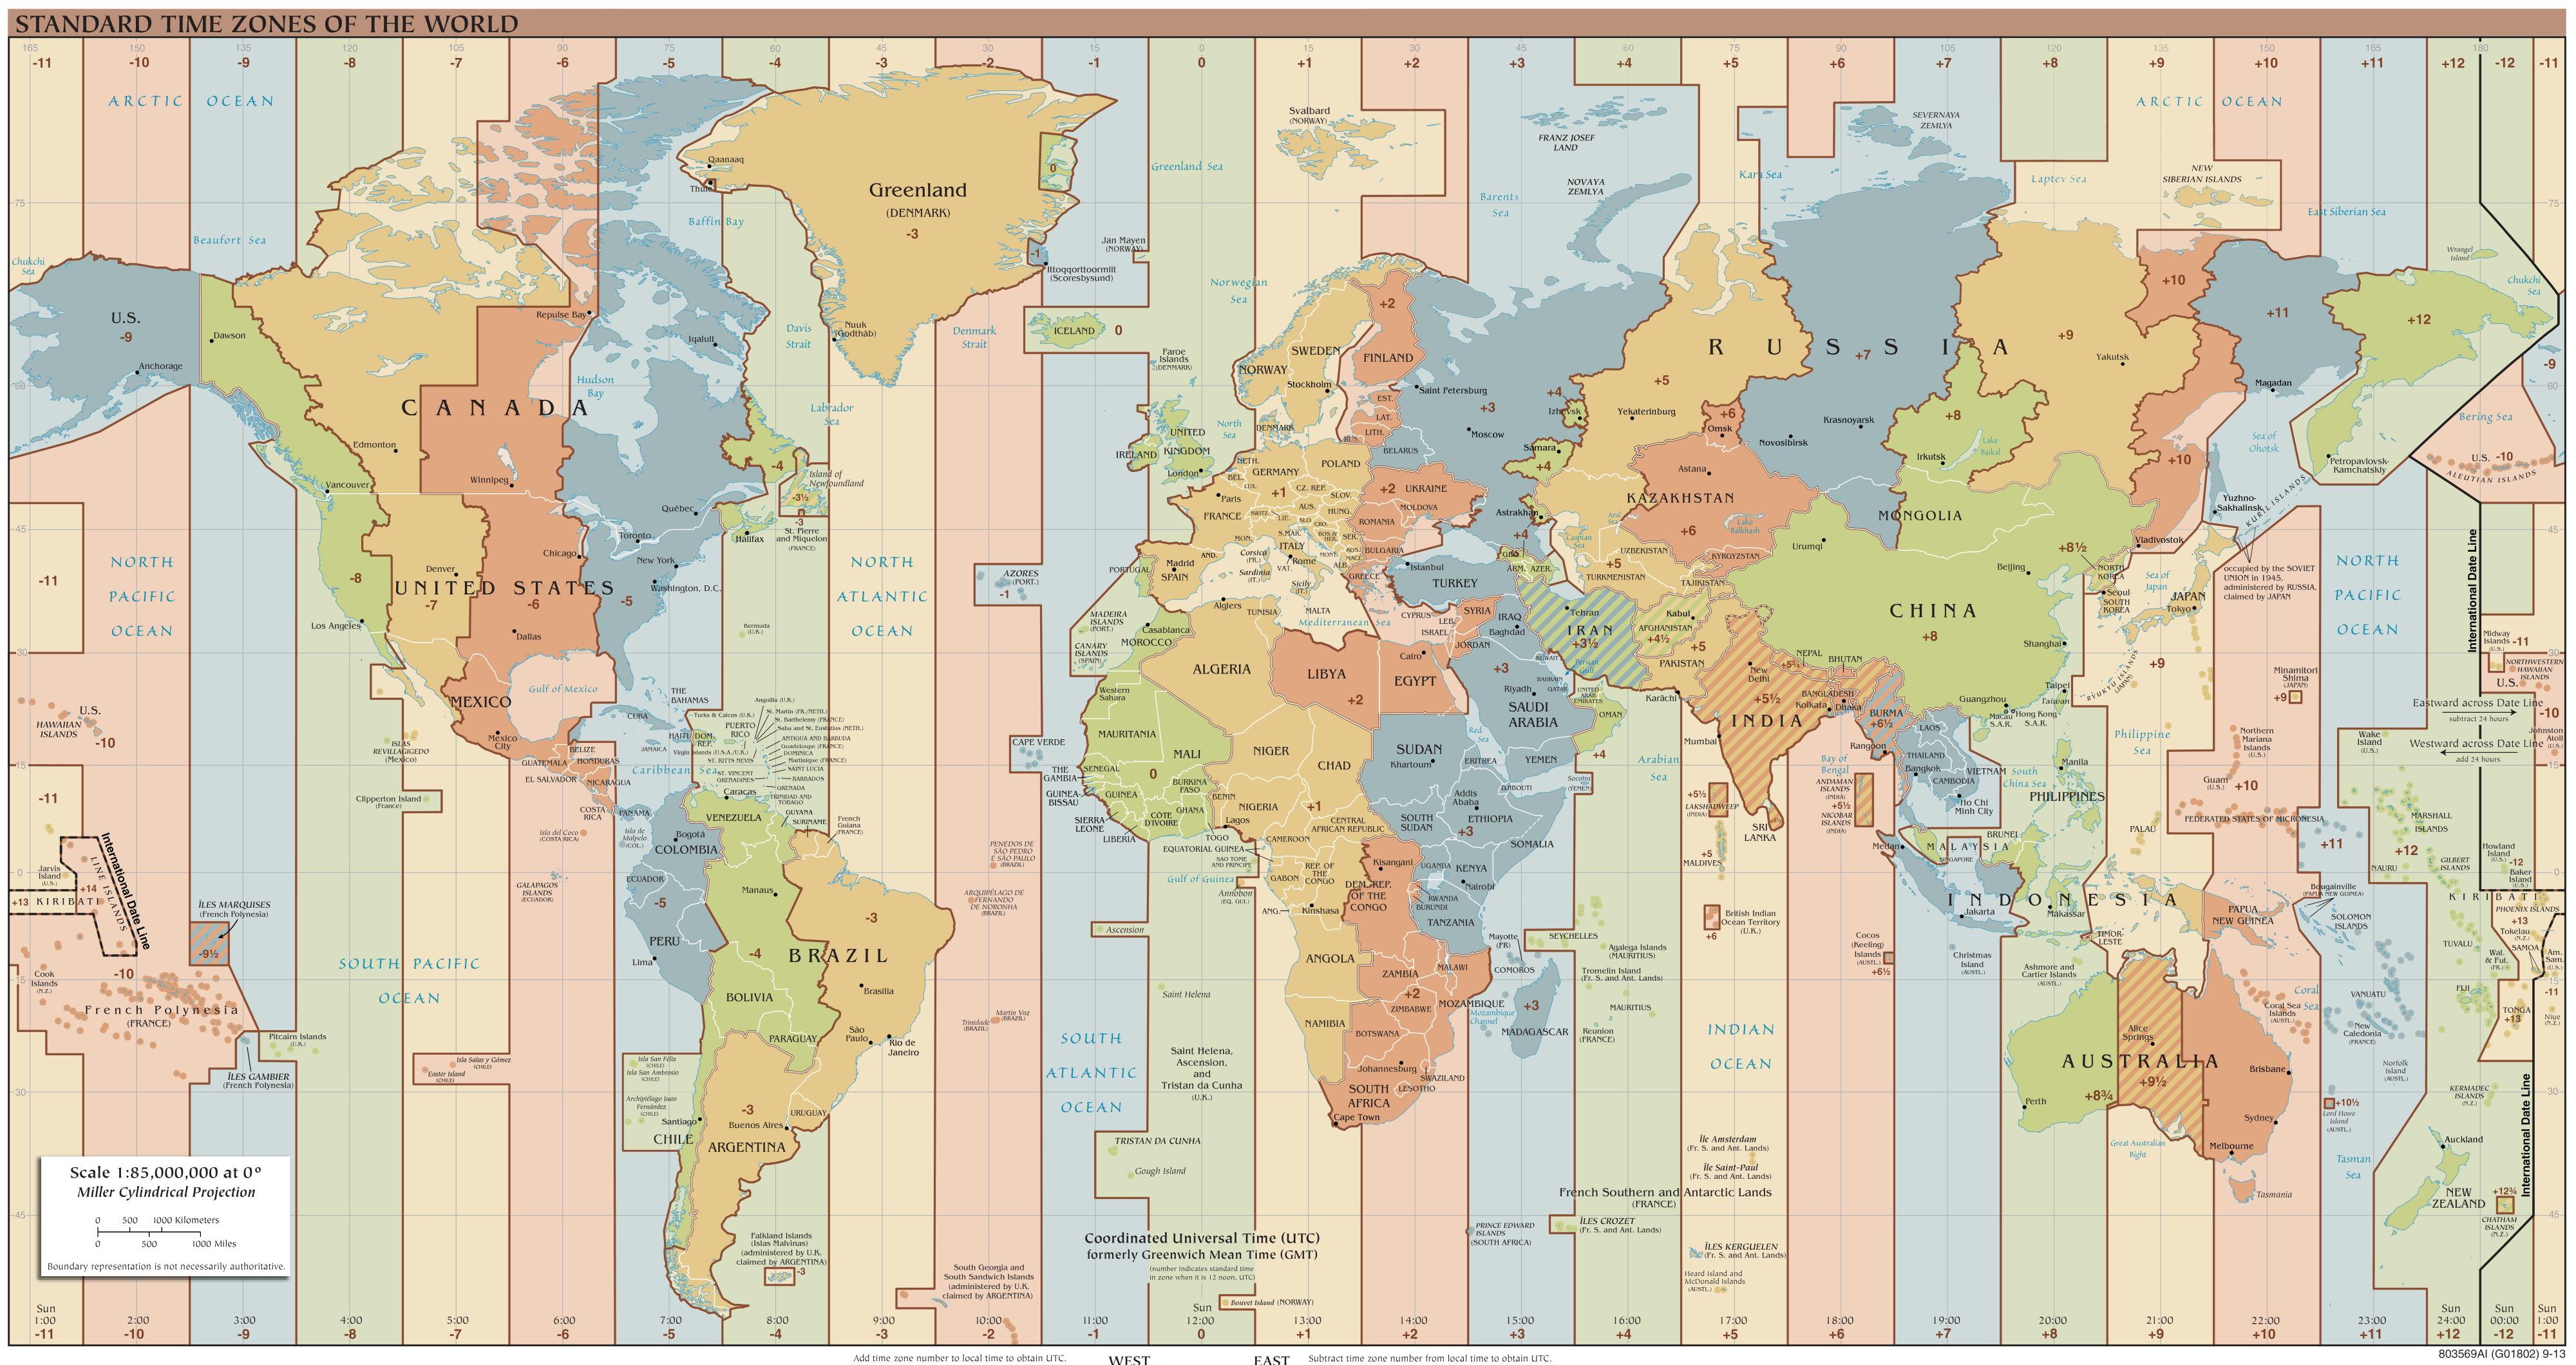
\includegraphics[width=0.95\textwidth]{images/std_time_zone.jpg}
        \caption{世界时区划分}
        \label{std_time_zone}
    \end{figure}

    \textbf{日界线}

    日界线是国际日期变更线的简称,为了统一日期的计时,在东十二区和西十二区附近设立的一条分界线。当从西向东跨过日界线时,日期加一天,从东向西跨过日界线时,日期减一天。
    \footnote{
        过日界线的计算:\url{https://zhuanlan.zhihu.com/p/250118987}
    }

    \begin{note}
        需要注意的是,日界线并不一定在东十二区和西十二区中间。
    \end{note}

    \subsection{ZoneId
        \footnote{
            JAVA8之 日期时间时区之 ZoneId[ZoneOffset, ZoneRegion] 笔记:\url{https://blog.csdn.net/kfepiza/article/details/115433132}
        }
    }

    \textbf{ZoneId}是在Java 1.8之后引入的时区Api,用于替代旧的Api \textbf{TimeZone},可以认为是一个区域的表示。

    \textbf{ZoneId}是一个抽象类,其有两个实现类:
    \begin{enumerate}
        \item \textbf{ZoneOffset} 该类为偏移时区,未指定具体区域。
        \item \textbf{ZoneRegion} 该类表示具体区域的时区。该类为internal。
    \end{enumerate}

    这三个类都没有公开构造函数,只能通过他们的静态方法去构建对象。\textbf{ZoneId}的静态方法可以构建出\textbf{ZoneOffset}或者\textbf{ZoneRegion}示例,而\textbf{ZoneOffset}的静态方法只能构建出\textbf{ZoneOffset}实例。\textbf{ZoneRegion}只能通过\textbf{ZoneId}的静态方法间接构造。

    下面给出了创建\textbf{ZoneId}的一些代码示例:

    \begin{lstlisting}[language=Kotlin]
@Test
fun testZoneIds() {
    // 0时区
    println(ZoneId.of("Z"))
    println(ZoneOffset.UTC)
    assertEquals(ZoneId.of("Z"), ZoneOffset.UTC)

    // UTC时区,需要注意的是ZoneId.of("UTC") != ZoneOffset.UTC
    println(ZoneId.of("UTC"))
    println(ZoneId.of("GMT"))
    
    // 系统默认时区,一般为Asia/Shanghai
    println(ZoneId.systemDefault())

    // UTC+8时区,下面四个方法是等价的
    println(ZoneId.of("+8"))
    println(ZoneId.of("+08:00"))
    println(ZoneOffset.of("+08:00"))
    println(ZoneOffset.ofHours(8))

    // Asia/Shanghai时区
    println(ZoneId.of("Asia/Shanghai"))
}
    \end{lstlisting}

    我们去研究\textbf{ZoneId}的代码,发现两个比较重要的抽象成员\textbf{id}和\textbf{rules}:

    \begin{lstlisting}[language=Kotlin]
public abstract class ZoneId implements Serializable {
    
    public abstract String getId();

    public abstract ZoneRules getRules();
}

    \end{lstlisting}

    其中\textbf{ZoneOffset}与\textbf{ZoneRegion}的实现如下:

    \begin{lstlisting}[language=Kotlin]
public final class ZoneOffset extends ZoneId implements TemporalAccessor, TemporalAdjuster, Comparable<ZoneOffset>, Serializable {
    
    /**
        Gets the normalized zone offset ID.
        The ID is minor variation to the standard ISO-8601 formatted string for the offset. There are three formats:
        Z - for UTC (ISO-8601)
        +hh:mm or -hh:mm - if the seconds are zero (ISO-8601)
        +hh:mm:ss or -hh:mm:ss - if the seconds are non-zero (not ISO-8601)
        Returns:
        the zone offset ID, not null
     */
    @Override
    public String getId() {
        return id;
    }
    
    /**
        Gets the associated time-zone rules.
        The rules will always return this offset when queried. The implementation class is immutable, thread-safe and serializable.
        Returns:
        the rules, not null
     */
    @Override
    public ZoneRules getRules() {
        return ZoneRules.of(this);
    }
}

final class ZoneRegion extends ZoneId implements Serializable {

    //-----------------------------------------------------------------------
    @Override
    public String getId() {
        return id;
    }

    @Override
    public ZoneRules getRules() {
        // additional query for group provider when null allows for possibility
        // that the provider was updated after the ZoneId was created
        return (rules != null ? rules : ZoneRulesProvider.getRules(id, false));
    }
}
    \end{lstlisting}

    我们可以发现\textbf{ZoneId}对应的具体时间偏移是存储在\textbf{rules}中的,由于该类的代码非常复杂,就不再深入研究了。同时,由于政策的因素,一个区域所属的时区可能随时发生变更。因此\textbf{ZoneRegion}的\textbf{rules}存储在系统资源中。

    \subsection{获取当前时间}

    我们首先看几个常用的Api获取当前时间的例子:

    \begin{lstlisting}[language=Kotlin]
@Test
fun testNow() {
    // Old Apis
    val oldDate = Date()
    println(oldDate)
    val oldDate2 = Calendar.getInstance().time
    println(oldDate2)

    // New Apis
    val instant = Instant.now()
    println(instant)

    val localDateTime = LocalDateTime.now()
    println(localDateTime)

    val zonedDateTime = Instant.now().atZone(ZoneId.systemDefault())
    println(zonedDateTime)
}
    \end{lstlisting}

    输入如下:(根据调用的时间会产生不同的结果)

    \begin{lstlisting}
Sun Jul 11 08:21:28 CST 2021
Sun Jul 11 08:21:28 CST 2021
2021-07-11T00:21:28.568046200Z
2021-07-11T08:21:28.583665900
2021-07-11T08:21:28.583665900+08:00[Asia/Shanghai]
    \end{lstlisting}

    可以发现\textbf{Instant.now()}获取的是当前的UTC时间,然后\textbf{LocalDateTime.now()}获取的是当前的本地时间。

    \begin{note}
        \textbf{CST}:区域Asia/Shanghai的简写

        \textbf{Date}获取的时间是不带时区信息的。在这五个对象的实例中,仅有\textbf{ZonedDateTime}带时区信息。
    \end{note}

    有一定了解的话,我们会发现\textbf{Date}的\textbf{hours}等属性是被废弃的,究其原因主要是其不自带时区信息,容易产生混淆。应当使用\textbf{Calandar}的相关方法进行代替。

    正式由于旧Api定义不明,使用复杂,精度不高。自java 1.8开始。\textbf{Instant}就替代了\textbf{Date},\textbf{LocalDateTime}、\textbf{ZonedDateTime}就替代了\textbf{Calandar},成为了java日期与时间的新的标准。

    \textbf{获得一个确定的时间}

    加入我们有一个时间2021/1/1 19:00:00(UTC),我们怎样通过新或者旧的Api去获取这个示例呢。下面给出几种调用的方式:

    \begin{lstlisting}[language=Kotlin]
@Test
fun testSpecific() {
    // 首先固定一个时钟 对应本地时间2021/7/12 3:00
    val fixedInstant = Instant.parse("2021-07-11T19:00:00.00Z")
    val fixedClock = Clock.fixed(
        fixedInstant, ZoneId.systemDefault()
    )

    val date = Date(fixedClock.millis())
    println(date)
    val date2 = Calendar.getInstance().apply {
        this.timeInMillis = fixedClock.millis()
    }.time
    println(date2)
    // 特别需要注意:Calendar.getInstance()会获取本地日历系统,设置的时间也是按照本地时间来设置的。
    val date3 = Calendar.getInstance().apply {
        this.set(Calendar.YEAR, 2021)
        // 特别需要注意的是,Calendar中Month范围为0~11.
        this.set(Calendar.MONTH, Calendar.JULY)
        this.set(Calendar.DATE, 12)
        this.set(Calendar.HOUR, 3)
        this.set(Calendar.MINUTE, 0)
        this.set(Calendar.SECOND, 0)
        // 这个一定要设置成0
        this.set(Calendar.MILLISECOND, 0)
    }.time
    println(date3)

    val date4 = Instant.from(fixedInstant)
    val date5 = Instant.ofEpochMilli(fixedClock.millis())
    println(date4)
    println(date5)

    val date6 = LocalDateTime.of(2021,7,12,3,0,0)
    println(date6)

    val date7 = ZonedDateTime.ofInstant(date4, ZoneId.systemDefault())
    println(date7)
}
    \end{lstlisting}

    输入如下:

    \begin{lstlisting}[]
Mon Jul 12 03:00:00 CST 2021
Mon Jul 12 03:00:00 CST 2021
Mon Jul 12 03:00:00 CST 2021
2021-07-11T19:00:00Z
2021-07-11T19:00:00Z
2021-07-12T03:00
2021-07-12T03:00+08:00[Asia/Shanghai]
    \end{lstlisting}

    \subsection{时间从哪来?时钟系统}

    如何获取当前的时间,就一定需要系统的相关资源,在阅读源码之后,我们会发现,无论是Old Api合适New Api,都是使用到时间戳,即相对于\textbf{EPOCH}的偏移量。

    \begin{note}
        在计算机系统中,会有一个时钟,用来记录距离1970-01-01T00:00:00Z(EPOCH)的毫秒数(或者纳秒数)。
    \end{note}

    我们先看两者源码的实现:

    \begin{lstlisting}[language=Kotlin]
public class Date implements java.io.Serializable, Cloneable, Comparable<Date>
{
    public Date() {
        this(System.currentTimeMillis());
    }
}

public final class Instant implements Temporal, TemporalAdjuster, Comparable<Instant>, Serializable {
    public static Instant now() {
        return Clock.systemUTC().instant();
    }
}

static final class SystemClock extends Clock implements Serializable {
    @Override
    public long millis() {
        // System.currentTimeMillis() and VM.getNanoTimeAdjustment(offset)
        // use the same time source - System.currentTimeMillis() simply
        // limits the resolution to milliseconds.
        // So we take the faster path and call System.currentTimeMillis()
        // directly - in order to avoid the performance penalty of
        // VM.getNanoTimeAdjustment(offset) which is less efficient.
        return System.currentTimeMillis();
    }
    @Override
    public Instant instant() {
        // Take a local copy of offset. offset can be updated concurrently
        // by other threads (even if we haven't made it volatile) so we will
        // work with a local copy.
        long localOffset = offset;
        long adjustment = VM.getNanoTimeAdjustment(localOffset);

        if (adjustment == -1) {
            // -1 is a sentinel value returned by VM.getNanoTimeAdjustment
            // when the offset it is given is too far off the current UTC
            // time. In principle, this should not happen unless the
            // JVM has run for more than ~136 years (not likely) or
            // someone is fiddling with the system time, or the offset is
            // by chance at 1ns in the future (very unlikely).
            // We can easily recover from all these conditions by bringing
            // back the offset in range and retry.

            // bring back the offset in range. We use -1024 to make
            // it more unlikely to hit the 1ns in the future condition.
            localOffset = System.currentTimeMillis()/1000 - 1024;

            // retry
            adjustment = VM.getNanoTimeAdjustment(localOffset);

            if (adjustment == -1) {
                // Should not happen: we just recomputed a new offset.
                // It should have fixed the issue.
                throw new InternalError("Offset " + localOffset + " is not in range");
            } else {
                // OK - recovery succeeded. Update the offset for the
                // next call...
                offset = localOffset;
            }
        }
        return Instant.ofEpochSecond(localOffset, adjustment);
    }
}
    \end{lstlisting}

    我们可以发现,两者通过逐级的调用,都使用到了\textbf{System.currentTimeMillis()},\\ \textbf{VM.getNanoTimeAdjustMent(Long)}两个方法,两者都是和硬件相关的。

    \textbf{Clock}
    
    Clock是在java1.8后引入的新的时钟类,主要用于提供当前的时间信息,实际上就是对系统资源的包装(Facade)。他具有四种实现类\textbf{SystemClock},\textbf{OffsetClock},\textbf{TickClock},
    \textbf{FixedClock}。
    
    其中\textbf{SystemClock}是系统时钟类,可以获取当前的时钟信息(系统资源)。而\textbf{FixedClock}提供一个固定的时钟,常常用于测试。其他的两个实现\textbf{OffsetClock}和\textbf{TickClock}都是装饰类,一个添加偏移,一个进行\textbf{truncate}操作。

    \subsection{Instant、LocalDateTime、ZoneDateTime之间的关系}

    \subsection{时间的属性获取与设置(Temporal)}

    \subsection{时间的加与减}

    \subsection{Duration与TemporalAmout}

    \section{Spring}

    \section{Locale}

    \section{NIO}



    \chapter{Record Logs}

    \section{2021年}

    \textbf{2021年7月10日} 创建了\ref{section_1}Joda-time时间处理类(since 1.8),编写第1-3节。
    
    \textbf{2021年7月11日} 编写\ref{section_1}Joda-time时间处理类(since 1.8)第4-5节。
    

\end{document}